\documentclass{article}

\usepackage{hyperref}
\usepackage{wrapfig}
\usepackage{graphicx}
\usepackage{tikz}
\usepackage{tikz-cd}

\usetikzlibrary{shapes,arrows, positioning,fit}

\title{Top}

\begin{document}

\noindent
\textbf{\Large Koji Sunami}
\hfill
\qquad
\href{https://kojisunami.github.io/index.html}{\textbf{Top}}
\qquad
\href{https://kojisunami.github.io/misc.html}{\textbf{Misc}}
\qquad
\href{https://kojisunami.github.io/cv-koji.pdf}{\textbf{CV}}



\noindent\rule{\textwidth}{0.4pt}

\begin{wrapfigure}{r}{0.25\textwidth}
    \centering
    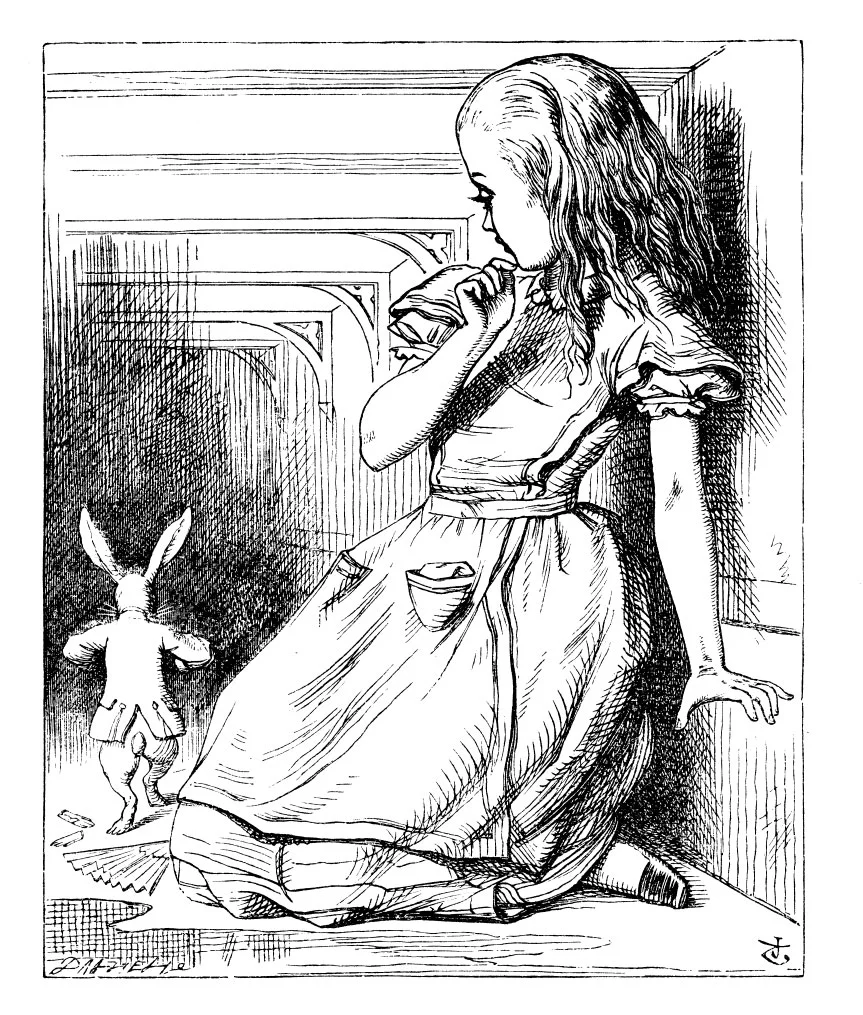
\includegraphics[width=0.2\textwidth]{alice1.png}
\end{wrapfigure}

\textbf{Research}

My interest in algebraic geometry is typically category / cohomology / homotopic and those of deformation,
I’d like to develop problems in Fukaya category, moduli problems, quotient stack, or any others. 
Here is a list of research proposals: \\

\newline

\begin{itemize}
\item \textbf{$A_\infty$-Enhancement of Geometry}  \\

\begin{wrapfigure}{r}{0.4\textwidth}
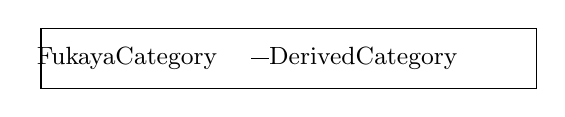
\begin{tikzpicture}[auto, every node/.style={font=\small}]
  \node (a) at (0,0) {Fukaya\\ Category};
  \node (b) at (3,0) {Derived\\ Category};
  \draw[-, shorten <= 15pt, shorten >= 3pt] (a) -- (b);
  \node[draw, rectangle, fit=(a) (b), inner xsep=10pt, xshift=15pt] {};
\end{tikzpicture}
\end{wrapfigure}

The proof of homological mirror symmetry conjecture is discussed from multi-dimensional perspective, 
including counting Gromow-Witten invariant, or Balmer spectrum, 
while generalizing formal geometry of non-unital $A_\infty$ algebra to $A_\infty$ category. 
\href{https://kojisunami.github.io/src/ainfty-geometry.pdf}{[link]} 

\item \textbf{Derived Intersection on Foliation} \\

\begin{wrapfigure}{r}{0.4\textwidth}
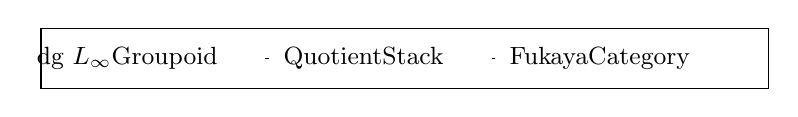
\begin{tikzpicture}[auto, every node/.style={font=\small}]
  \node (a) at (0,0) {dg $L_\infty$\\ Groupoid};
  \node (b) at (3,0) {Quotient\\ Stack};
  \node (c) at (6,0) {Fukaya\\ Category};
  \draw[-, shorten <= 15pt, shorten >= 3pt] (a) -- (b);
  \draw[-, shorten <= 15pt, shorten >= 3pt] (b) -- (c);
  \node[draw, rectangle, fit=(a) (b) (c), inner xsep=10pt, xshift=15pt] {};
\end{tikzpicture}
\end{wrapfigure}

Derived algebraic geometry proves the $\infty$-equivalence of dg Lie algebroid and foliation. Now the quotient is defined by quotient of dg 
$L_\infty$ groupoid generated from dg Lie algebroid, and it’s calculated by dg $L_\infty$ version of Chevalley-Eilenberg complex.
I'm also wondering evaluation of the foliation using language of DT/GW invariants.
\href{https://kojisunami.github.io/src/dgla-stack.pdf}{[link]}  

\end{itemize}



\noindent\rule{\textwidth}{0.4pt}


\begin{wrapfigure}{r}{0.25\textwidth}
    \centering
    
\includegraphics[width=0.2\textwidth]{alice2.png}
\end{wrapfigure}

\noindent
\textbf{Exposition} \\

This is a list of pdf previously shown to other people or intended to be distributed in the future.

\newline
\newline
\newline

\begin{itemize}
\item \textbf{What is Math?} \\
This is ideally for everybody, who are doubting the purpose of math higher than calculus and linear algebra. 
The tone of the argument is describing the process of how the high school math jump into the research math.
\href{https://kojisunami.github.io/src/what-math.pdf}{[link]}

\item \textbf{(Spring 2026) Intro to Deformation} \\
DAG stands from AG + deformation. $\infty$-language. [link]

\item \textbf{(Fall 2022) Cheat Cheet Mirror Symmetry} \\
Marc Gross’s tropical/toric geometry and quantum cohomology for mirror symmetry. It’s for exam for PhD Candidate.
\href{https://kojisunami.github.io/study_notes/qe2-major-ver3.pdf}{[link]}

\item \textbf{(Fall 2022), Intro to Geometric Satake Correspondence} \\
Grand relationship among AG, RT, and NT.
\href{https://kojisunami.github.io/study_notes/satake-ver2.pdf}{[link]}

\item \textbf{(Winter 2019) Brown Representability} \\
Introducing Brown representability in triangulated category. It’s bachelor’s thesis.
\href{https://kojisunami.github.io/study_notes/brt.pdf}{[link]}
\end{itemize}



\noindent\rule{\textwidth}{0.4pt}


\begin{wrapfigure}{r}{0.25\textwidth}
    \centering
    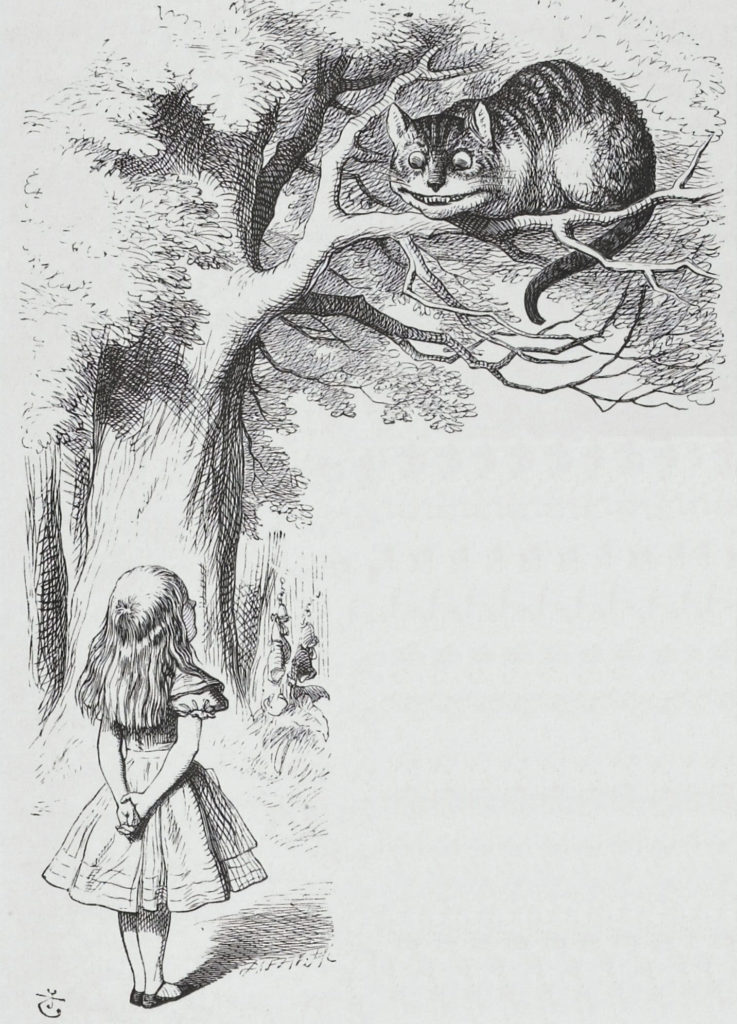
\includegraphics[width=0.2\textwidth]{alice3.png}
\end{wrapfigure}

\noindent
\textbf{Casual Non-Research Interests} \\

Below is the list of materials I personally think interesting, and they are somewhat connecting to algebraic geometry. 
They are quite different from my focus, however.

\newline

\begin{itemize}
\item \textbf{AdS/CFT} \\
AdS/CFT claims the correspondence of the boundaries not only the shape but also the behavior on it of both AdS and CFT, 
even though AdS and CFT are mathematically very different structures. The phenomena on the boundary is called holography. 
Ryu-Takayanagi induces the formula of quantum-entanglement from AdS/CFT correspondence. 
Meanwhile, CFT itself can derive a variety of Non-linear PDE in particular Navier-Stokes equation, 
and AdS is modeled algebraic geometrically using Sasaki-Einstein.

\item \textbf{Spin(7) Geometry and M-theory} \\
The benefit of generalizing superstring theories to M-theory is efficiating computation of perturbation effect, while M-theory is generating 
$G_2$ holonomy in 11-dimensional space. Joyce conjecture claims moduli space of coassociative submanifold of 
$G_2$ bundle contains symplectic structure.

\item \textbf{Geometric Langlands} \\
Geometric Langlands is a duality connecting local system and D-module and Higgs bundle, and this is not number theory.  
4d CFT derives Higgs bundle through Kapustin-Witten, whose S-duality is D-module.
\end{itemize}



\noindent\rule{\textwidth}{0.4pt}

\noindent
\textbf{My Education-Research Interest} \\

The bias of my interest in education is to make people interested in algebraic geometry and math physics.
The importance of algebraic geometry is increasing year by year. 
In math physics, it was QFT in 1950s and string theory in 1980s, floer and Chern-Simon in 1980s, mirror symmetry and S-duality in 1990s,
M theory in 2000s, where all of them are somewhat heavily algebraic geometry, 
and in 2026 at present, this area of study is still developing today.

\begin{itemize}
\item Infty category argument is hard to read by symbolic mean, because everything looks the same. I want to improve the readability.
\item Argument of something without actually knowing the technical detail. 
If smart high school student can discuss something of string theory by seeing TV's documentary, 
can we do the same with algebraic geometry or math physics?
\item How to make college students interested in pure math, assuming they know calculus and linear algebra.
\item How to write better
\end{itemize}


 
\noindent\rule{\textwidth}{0.4pt}


\begin{wrapfigure}{r}{0.25\textwidth}
    \centering
    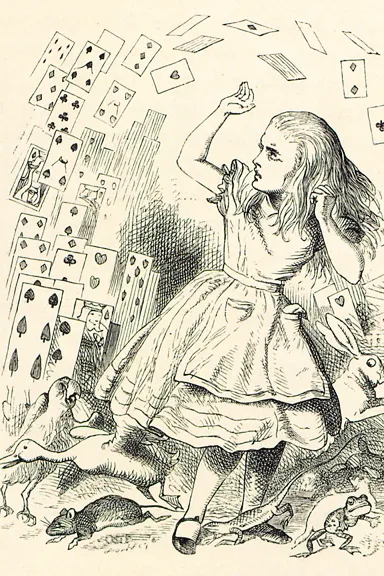
\includegraphics[width=0.2\textwidth]{alice4.png}
\end{wrapfigure}

\noindent
\textbf{Junk} \\

I have invented two junk pdf of totally approximatelly 200 pages based on rabbit holing ChatGPT or wikipedia for a period of time.
It helped to more focus on the purpose of study by cultivating my broad interests in math.
Perhaps, quantity surpasses quality to cultivate math maturity,
as analogy in football, running, dribbling and shooting is more fundamental than the technical stuff.

\begin{itemize}
\item \textbf{(Spring 2026) Intro to Geometry} \\
Post-Hartshorne NC alg/diff geometry. Prelim for reading mirror symmetry papers.
\href{https://kojisunami.github.io/study_notes/geometry-intro.pdf}{[link]}

\item \textbf{(Fall 2025) Intro to Math Physics} \\
QFT, string theory, mirror symmetry and AdS/CFT, beginning from classical. 
\href{https://kojisunami.github.io/study_notes/physics-intro.pdf}{[link]}
\end{itemize}



\end{document}
